\section{Аналитические раздел}

\subsection{Принцип $\Delta t$}

Принцип $\Delta t$ заключается в последовательном анализе состояний всех блоков 
в момент $t + \Delta t$ по заданному состоянию блоков в момент $t$. 
При этом новое состояние блоков определяется в соответствии с их алгоритмическим 
описанием с учетом действующих случайных факторов, задаваемых распределениями 
вероятности. 

В результате принимается решение о том, какие общесистемные события 
должны имитироваться программной моделью на данный момент времени. 
Основной недостаток: значительные затраты машинного времени на реализацию 
моделирования системы. При недостаточно малом $\Delta t$ появляется опасность 
пропуска отдельных событий в системе, что исключает возможность получения 
адекватных результатов при моделировании. 
К достоинствам относится равномерная протяжка времени.

\subsection{Событийный принцип}

При использовании событийного принципа, 
состояние всех блоков имитационной модели анализируется лишь 
в момент появления какого-либо события. Момент поступления 
следующего события определяется минимальным значением из списка будущих событий, 
представляющего собой совокупность моментов ближайшего изменения состояния 
каждого из блоков системы.


\section{Результаты работы}

Условием остановки поиска --- обслуживание 1000 сообщений без
изменения максимальной длины очереди. Если такое событие не происходит за $10^5$
заявок, принимается, что генерация вместе с обратной связью помещают
сообщения с большей интенсивностью, чем успевает обрабатывать их
обслуживающий автомат. Со временем длина очереди будет только расти,
поэтому для любой выбранной очереди в определенный момент произойдут
потери.

На рисунке \ref{fig:r2} редставлен результат работы программы при различных параметрах.

\begin{figure}[ht!]
	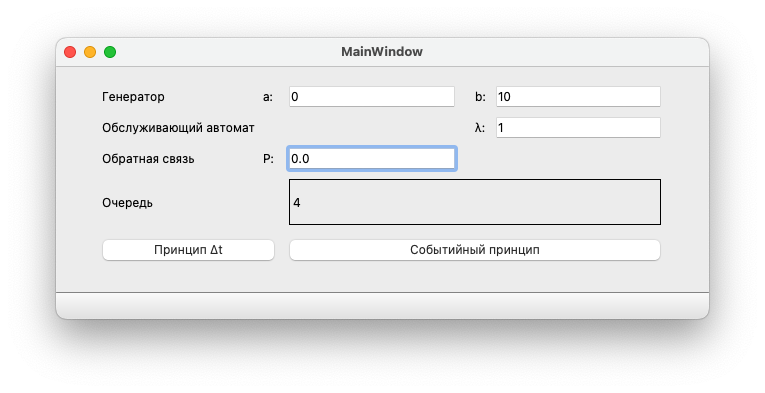
\includegraphics[width=0.75\linewidth]{assets/images/res.png}
	\caption{Система при более интенсивном обслуживании}
	\label{fig:r2}
\end{figure}